\documentclass[ngerman,hyperref={pdfpagelabels=false}]{beamer}

% -----------------------------------------------------------------------------

\graphicspath{{images/}}

% -----------------------------------------------------------------------------

\usetheme{KIT}

\setbeamercovered{transparent}
%\setbeamertemplate{enumerate items}[ball]

\newenvironment<>{KITtestblock}[2][]
{\begin{KITcolblock}<#1>{#2}{KITblack15}{KITblack50}}
{\end{KITcolblock}}

\usepackage[ngerman,english]{babel}
\usepackage[utf8]{inputenc}
\usepackage[TS1,T1]{fontenc}
\usepackage{array}
\usepackage{multicol}
\usepackage[absolute,overlay]{textpos}
\usepackage{beamerKITdefs}

\pdfpageattr {/Group << /S /Transparency /I true /CS /DeviceRGB>>}	%required to prevent color shifting withd transparent images


\title{Kolloqium Planungsphase}
\subtitle{Team B}

\author[Team B]{Team B}
\institute{Institut für Programmierparadigmen}

\TitleImage[width=\titleimagewd,height=\titleimageht]{titel}

\KITinstitute{Institut f\"ur Programmierparadigmen}
\KITfaculty{Fakult\"at f\"ur Informatik}

% -----------------------------------------------------------------------------

\begin{document}
\setlength\textheight{7cm} %required for correct vertical alignment, if [t] is not used as documentclass parameter


% title frame
\begin{frame}
  \maketitle
\end{frame}


% ---------------
% Vorstellung
% ---------------

\section{Vorstellung}
\begin{frame}
	\frametitle{Vorstellung Team B}
	\begin{itemize}
		\item Luca Becker, Henrike Hardt, Larissa Schmid, Adrian Schulte, Maik Wiesner
		\item PSE-Projekt: Lambda - Das Spiel
	\end{itemize}
	\bigskip
\end{frame}


% ---------------
% Spielidee
% ---------------

\section{Spielidee}
\begin{frame}
	\frametitle{Spielidee}
	\begin{itemize}
		\item Jump 'N' Run-Stil
		\item Spielerische Verdeutlichung des $\lambda$-Kalküls durch Maschinen und Metallobjekte, die platziert werden müssen
		\item Abstrakte Darstellung sorgt für mehr Spielspaß
	\end{itemize}	
\end{frame}



% ---------------
% Levelbeispiel
% ---------------

\section{Levelbeispiel}

\subsection{Lambda-Kalkül}
\begin{frame}
	\frametitle{Levelbeispiel}
	\framesubtitle{$\lambda$-Kalkül}	
	\huge{\[(\lambda x.(\lambda f.(f \circ f))(\lambda y.y)(x))(2)\]}
\end{frame}

\subsection{Levelstart}
\begin{frame}
	\frametitle{$\lambda$-Ausdruck in unserem Spiel}
	
	\begin{columns}[T]
		\begin{column}[T]{5cm} 
			Levelstart:\\
		\end{column}
		\begin{column}[T]{5cm}
			%Bild von achtem Schritt
		\end{column}
		\end{columns}
	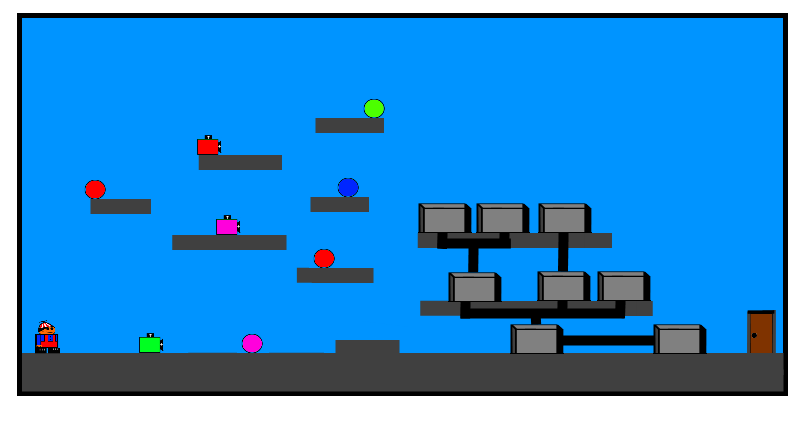
\includegraphics[scale= 0.55]{images/Levelbeginn}
\end{frame}

\subsection{Objekte bewegen}
\begin{frame}
	\frametitle{Elemente bewegen}
	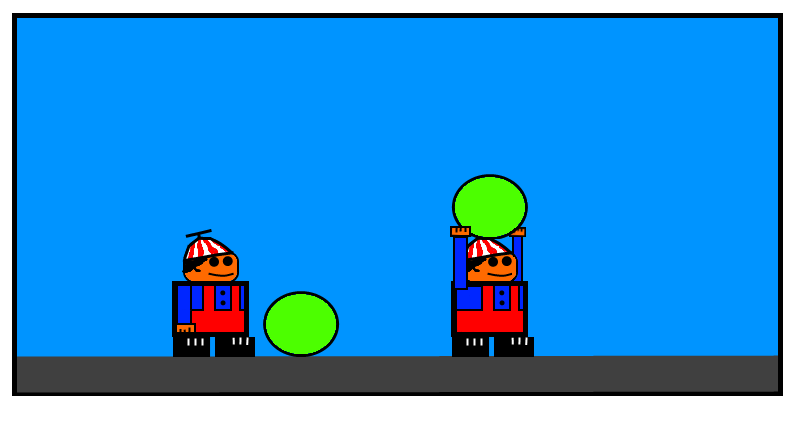
\includegraphics[scale= 0.55]{images/AufnehmenAblegenR}
\end{frame}

\subsection{Levelende}
\begin{frame}
	\frametitle{$\lambda$-Ausdruck in unserem Spiel}
	
	\begin{columns}[T]
		\begin{column}[T]{5cm} 
			Levelende:\\
		\end{column}
		\begin{column}[T]{5cm}
			%Bild von achtem Schritt
		\end{column}
		\end{columns}
	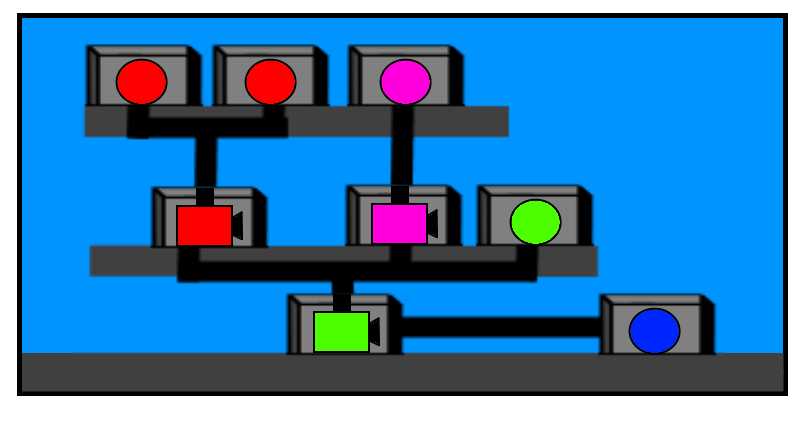
\includegraphics[scale= 0.55]{images/Levelende}
\end{frame}

\subsection{Auswertung}

\begin{frame}
	\frametitle{$\lambda$-Ausdruck in unserem Spiel}
	\begin{columns}[T]
		\begin{column}[T]{5cm} 
			Beginn Auswertung:\\
		\end{column}
		\begin{column}[T]{5cm}
			%Bild von achtem Schritt
		\end{column}
		\end{columns}
	
	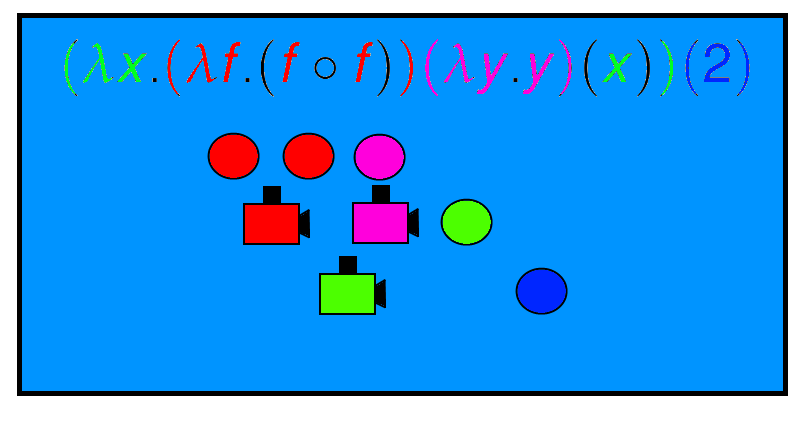
\includegraphics[scale= 0.55]{images/Auswertung1mA}
\end{frame}

\begin{frame}{Auswertung des $\lambda$-Ausdrucks}
	%\frametitle{Auswertung des $\lambda$-Ausdrucks}
	\begin{columns}[T]
		\begin{column}[T]{5cm} 
		     \[(\lambda f.(f \circ f))(\lambda y.y)(x)
		     [x \leftarrow 2]\]
		\end{column}
		\begin{column}[T]{5cm}
			
		\end{column}
	\end{columns}
	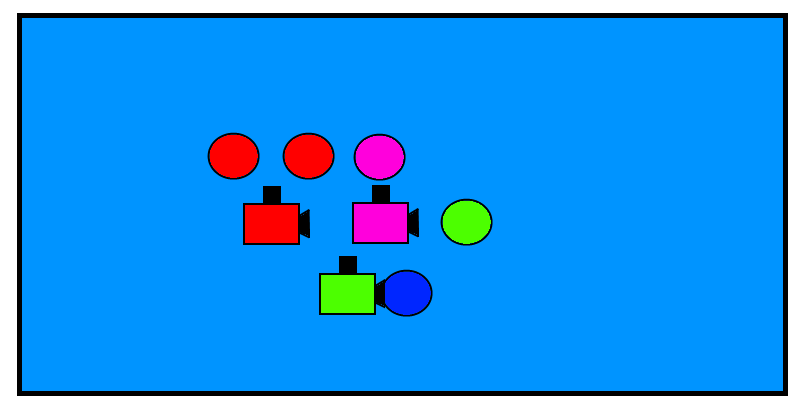
\includegraphics[scale= 0.55]{images/Auswertung2}
\end{frame}


\begin{frame}{Auswertung des $\lambda$-Ausdrucks}
	%\frametitle{Auswertung des $\lambda$-Ausdrucks}
	\begin{columns}[T]
		\begin{column}[T]{5cm} 
			\[(\lambda f.(f \circ f))(\lambda y.y)(x)[x \leftarrow 2]\]
		\end{column}
		\begin{column}[T]{5cm}
			
		\end{column}
	\end{columns}
	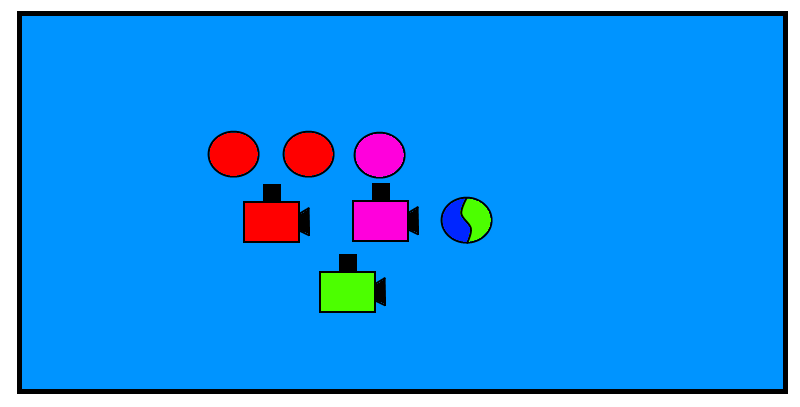
\includegraphics[scale= 0.55]{images/Auswertung3}
\end{frame}



\begin{frame}{Auswertung des $\lambda$-Ausdrucks}
		\begin{columns}[T]
			\begin{column}[T]{5cm} 
				\[(\lambda f.(f \circ f))(\lambda y.y)(2)\]
			\end{column}
			\begin{column}[T]{5cm}
				%Bild von zweitem Schritt
			\end{column}
		\end{columns}	
		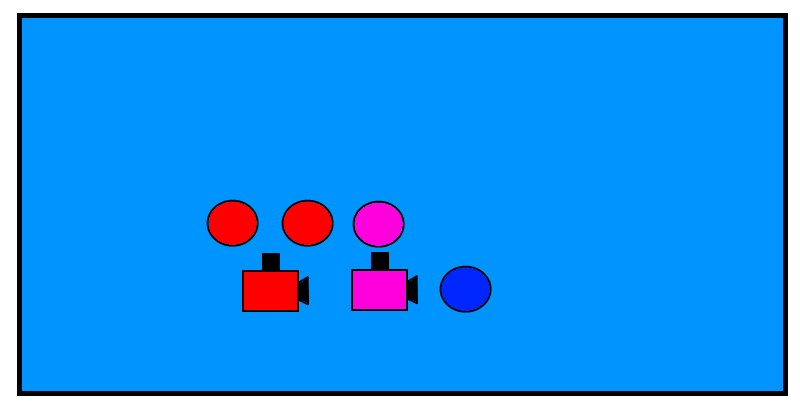
\includegraphics[scale= 0.55]{images/Auswertung4}
\end{frame}


\begin{frame}{Auswertung des $\lambda$-Ausdrucks}
	\begin{columns}[T]
		\begin{column}[T]{5cm} 
			\[(f \circ f)[f \leftarrow \lambda y.y](2)\]
		\end{column}
		\begin{column}[T]{5cm}
			%Bild von drittem Schritt
		\end{column}
	\end{columns}
	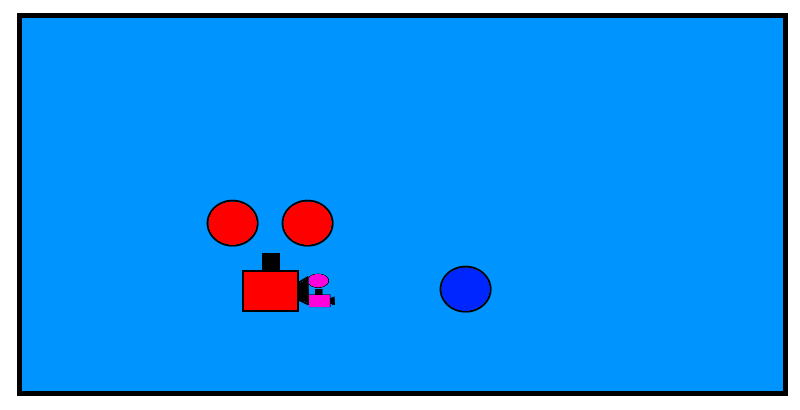
\includegraphics[scale= 0.55]{images/Auswertung5}
\end{frame}

\begin{frame}{Auswertung des $\lambda$-Ausdrucks}
	\begin{columns}[T]
		\begin{column}[T]{5cm} 
			\[(f \circ f)[f \leftarrow \lambda y.y](2)\]
		\end{column}
		\begin{column}[T]{5cm}
			%Bild von drittem Schritt
		\end{column}
	\end{columns}
	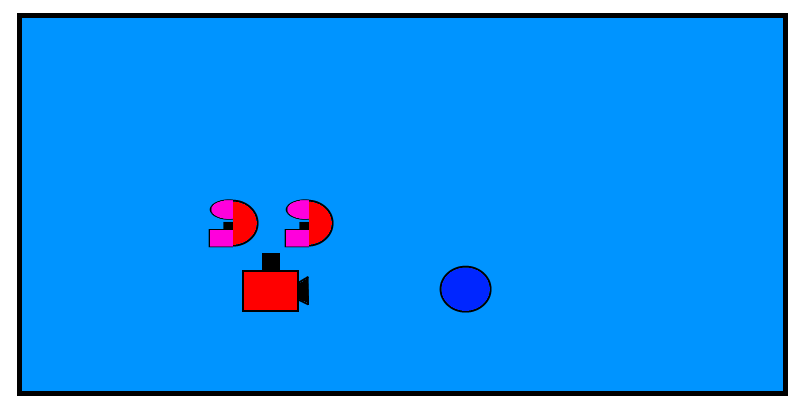
\includegraphics[scale= 0.55]{images/Auswertung6}
\end{frame}


\begin{frame}{Auswertung des $\lambda$-Ausdrucks}
	\begin{columns}[T]
		\begin{column}[T]{5cm} 
			\[((\lambda y.y)(\lambda y.y))(2)\]
		\end{column}
		\begin{column}[T]{5cm}
			%Bild von viertem Schritt
		\end{column}
	\end{columns}
	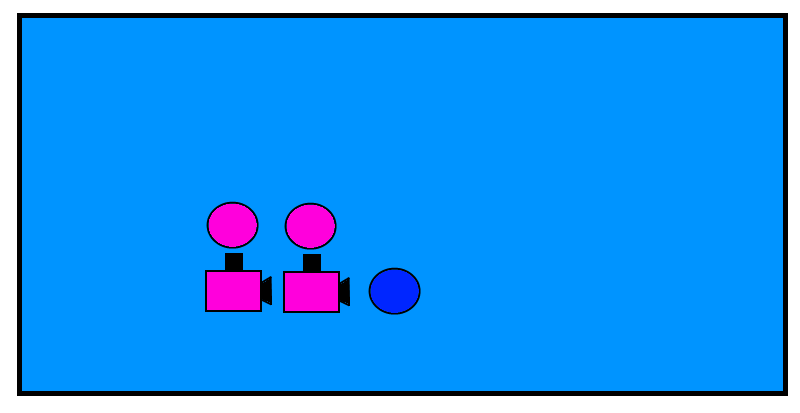
\includegraphics[scale= 0.55]{images/Auswertung7}
\end{frame}


\begin{frame}{Auswertung des $\lambda$-Ausdrucks}
	%\frametitle{Auswertung des $\lambda$-Ausdrucks}
	\begin{columns}[T]
		\begin{column}[T]{5cm} 
			\[(y[y \leftarrow (\lambda y.y)])(2)\]
		\end{column}
		\begin{column}[T]{5cm}
			%Bild von fünftem Schritt
		\end{column}
	\end{columns}
	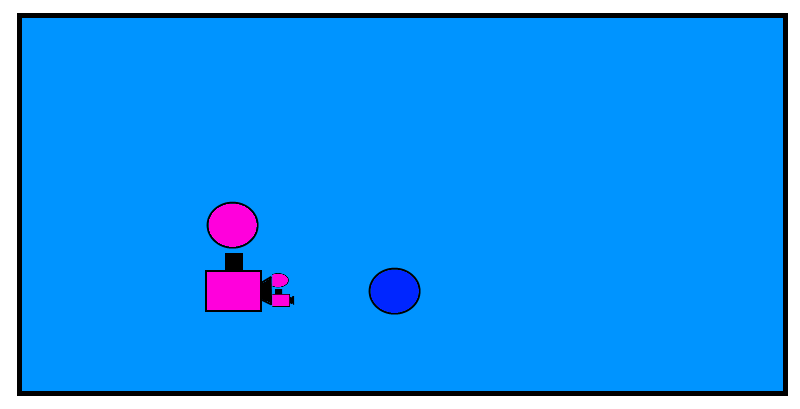
\includegraphics[scale= 0.55]{images/Auswertung8}
\end{frame}

\begin{frame}{Auswertung des $\lambda$-Ausdrucks}
	%\frametitle{Auswertung des $\lambda$-Ausdrucks}
	\begin{columns}[T]
		\begin{column}[T]{5cm} 
			\[(y[y \leftarrow (\lambda y.y)])(2)\]
		\end{column}
		\begin{column}[T]{5cm}
			%Bild von fünftem Schritt
		\end{column}
	\end{columns}
	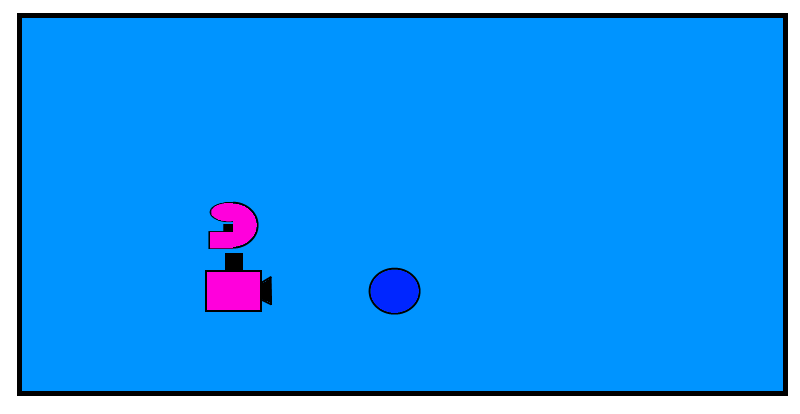
\includegraphics[scale= 0.55]{images/Auswertung9}
\end{frame}


\begin{frame}{Auswertung des $\lambda$-Ausdrucks}
	%\frametitle{Auswertung des $\lambda$-Ausdrucks}
	\begin{columns}[T]
		\begin{column}[T]{5cm} 
			\[(\lambda y.y)(2)\]
		\end{column}
		\begin{column}[T]{5cm}
			%Bild von sechstem Schritt
		\end{column}
	\end{columns}
	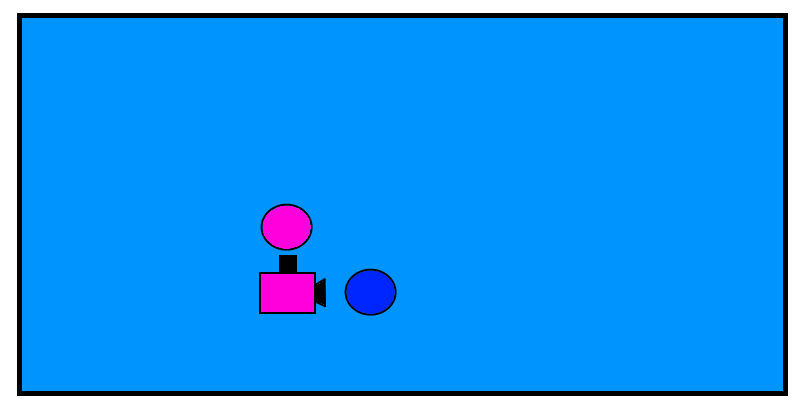
\includegraphics[scale= 0.55]{images/Auswertung10}
\end{frame}


\begin{frame}{Auswertung des $\lambda$-Ausdrucks}
	%\frametitle{Auswertung des $\lambda$-Ausdrucks}
	\begin{columns}[T]
		\begin{column}[T]{5cm} 
			\[y[y \leftarrow 2]\]
		\end{column}
		\begin{column}[T]{5cm}
			%Bild von siebtem Schritt
		\end{column}
	\end{columns}
	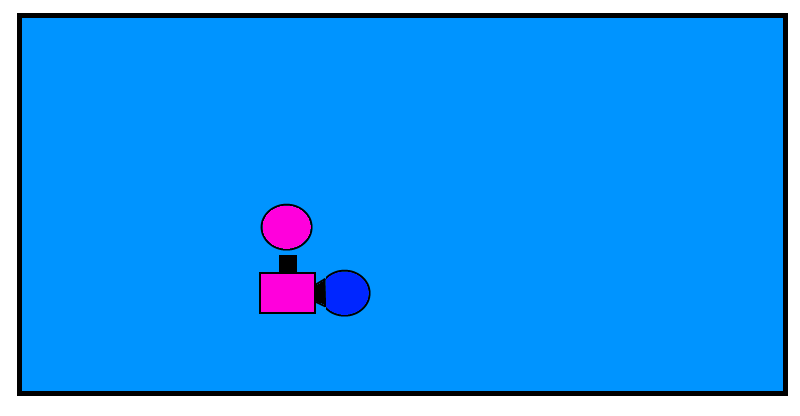
\includegraphics[scale= 0.55]{images/Auswertung11}
\end{frame}

\begin{frame}{Auswertung des $\lambda$-Ausdrucks}
	%\frametitle{Auswertung des $\lambda$-Ausdrucks}
	\begin{columns}[T]
		\begin{column}[T]{5cm} 
			\[y[y \leftarrow 2]\]
		\end{column}
		\begin{column}[T]{5cm}
			%Bild von siebtem Schritt
		\end{column}
	\end{columns}
	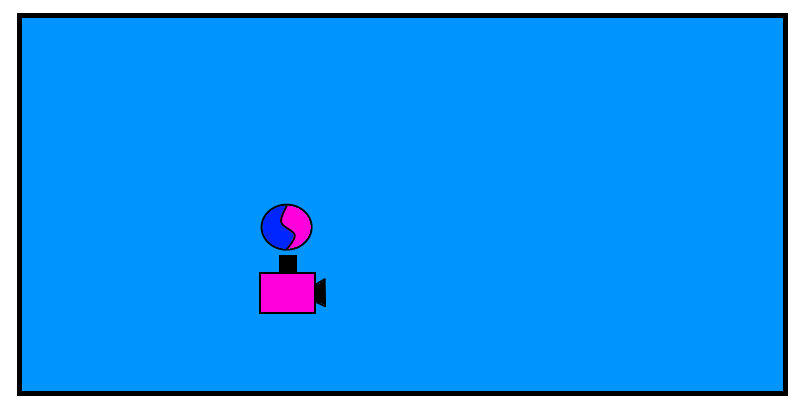
\includegraphics[scale= 0.55]{images/Auswertung12}
\end{frame}


\begin{frame}{Auswertung des $\lambda$-Ausdrucks}
	%\frametitle{Auswertung des $\lambda$-Ausdrucks}
	\begin{columns}[T]
		\begin{column}[T]{5cm} 
			\[2\]
		\end{column}
		\begin{column}[T]{5cm}
			%Bild von achtem Schritt
		\end{column}
	\end{columns}
	
\includegraphics[scale= 0.55]{images/Auswertung13}
\end{frame}

\begin{frame}{Auswertung des $\lambda$-Ausdrucks}
	%\frametitle{Auswertung des $\lambda$-Ausdrucks}
	\begin{columns}[T]
		\begin{column}[T]{5cm} 
			Levelausgang:
		\end{column}
		\begin{column}[T]{5cm}
			%Bild von achtem Schritt
		\end{column}
	\end{columns}
	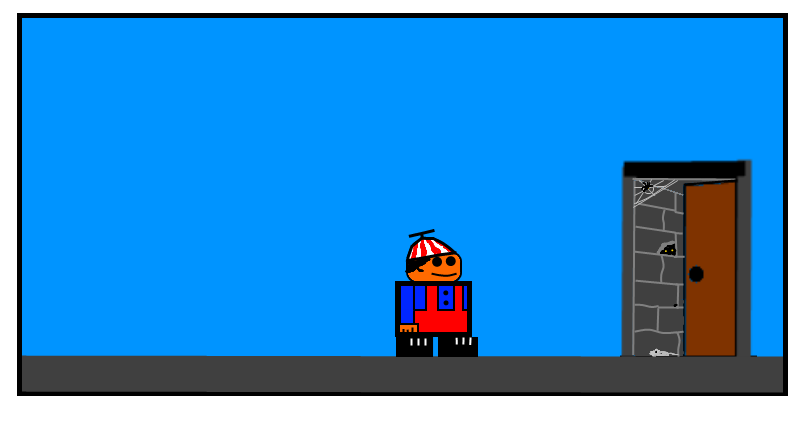
\includegraphics[scale= 0.55]{images/Levelausgang}
\end{frame}

% ---------------
% Kriterien
% ---------------

\section{Kriterien}

\subsection{Musskriterien}
\begin{frame}
	\frametitle{Kriterien}
	\framesubtitle{Musskriterien}
	\begin{itemize}
		\item Spielerisches Vermitteln des $\lambda$-Kalküls
		\item Nach dem Wasserfall-Modell erarbeitetes Spiel
		\item Touch-Bedienung
		\item mindestens fünf individuelle Level
	\end{itemize}
\end{frame}

\subsection{Wunschkriterien}
\begin{frame}
	\frametitle{Kriterien}
	\framesubtitle{Wunschkriterien}
	\begin{itemize}
		\item Retrolook
		\item Mehrere Spielmodi
		\item Begleitende Story
		\item Erweiternde Spiel- und Levelelemente
		\item Challengemode mit Zeitdruck
	\end{itemize}
\end{frame}

\subsection{Abgrenzngskriterien}
\begin{frame}
	\frametitle{Kriterien}
	\framesubtitle{Abgrenzungskriterien}
	\begin{itemize}
		\item Kein Mehrspieler-Modus
		\item Keine Online-Anbindung
		\item Keine Kompatibilität mit anderen Geräten/Betriebssystemen ohne Emulation
	\end{itemize}
\end{frame}



\begin{frame}
	\huge
	Vielen Dank für Ihre Aufmerksamkeit!
\end{frame}

\end{document}
